\documentclass{beamer}
\usepackage[english, russian]{babel}
\usepackage[T2A]{fontenc}
\usepackage[utf8]{inputenc}
\usepackage{indentfirst}
\usepackage{amsmath, amsfonts, amssymb, amsthm, mathtools}
\usepackage[export]{adjustbox}
\usepackage{graphicx} 
\graphicspath{ {./images/} }

\usepackage{subcaption}
\usepackage{verbatim}

\usepackage{minted}{\setlength{\parskip}{0pt}}

\usepackage{hyperref}

\hypersetup{
    colorlinks=true,
    linkcolor=blue,
    filecolor=magenta,      
    urlcolor=black,
    pdftitle={Overleaf Example},
    pdfpagemode=FullScreen,
    }


\title{Лабораторная работа № 9. \\ Настройка POP3/IMAP сервера}
\author{Данила Стариков \\ НПИбд-02-22}
\institute{Российский университет дружбы народов имени Патриса Лумумбы}
\date{2024}

\begin{document}

\frame{\titlepage}

\begin{frame}
\frametitle{Цель работы}
\begin{itemize}
    \item Приобретение практических навыков по установке и простейшему конфигурированию POP3/IMAP-сервера
\end{itemize}
\end{frame}

\begin{frame}[fragile]
  \frametitle{Установка Dovecot}
Установили на сервере необходимые для работы пакеты:
\begin{minted}{bash}
    dnf -y install dovecot telnet
\end{minted}
\end{frame}

\begin{frame}
\frametitle{Настройка Dovecot}
    \centering
    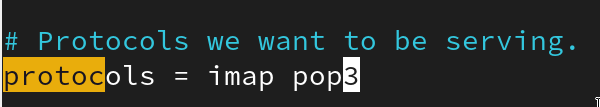
\includegraphics[width=\textwidth]{../images/image01.png}
    \captionof{figure}{Разрешенные почтовые протоколы в конфигурации Dovecot.}
\end{frame}

\begin{frame}
\frametitle{Настройка Dovecot}
    \centering
    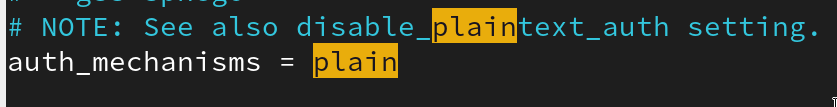
\includegraphics[width=\textwidth]{../images/image02.png}
    \captionof{figure}{Указание метода аутентификации \texttt{plain}.}
\end{frame}

\begin{frame}
\frametitle{Настройка Dovecot}
    \centering
    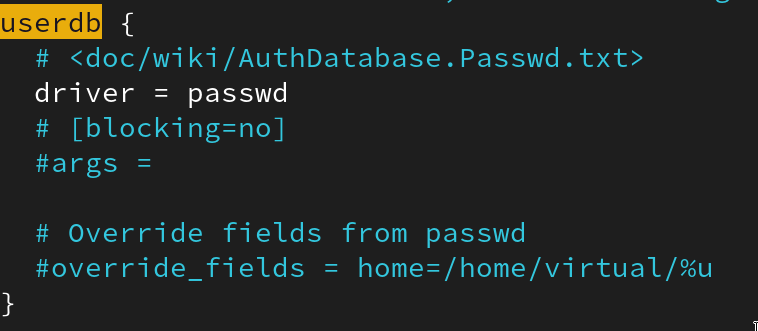
\includegraphics[width=\textwidth]{../images/image03.png}
    \captionof{figure}{Использование файла \texttt{passwd} для поиска паролей.}
\end{frame}

\begin{frame}
\frametitle{Настройка Dovecot}
    \centering
    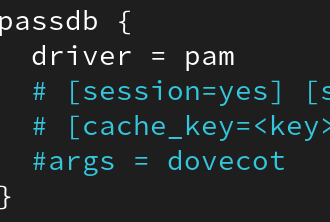
\includegraphics[width=\textwidth]{../images/image04.png}
    \captionof{figure}{Использование \texttt{pam} пользователей.}
\end{frame}

\begin{frame}
\frametitle{Настройка Dovecot}
    \centering
    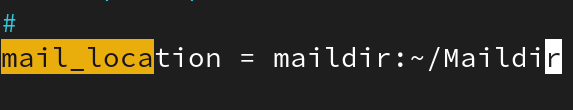
\includegraphics[width=\textwidth]{../images/image05.png}
    \captionof{figure}{Настройка месторасположения почтовых ящиков пользователей.}
\end{frame}
\begin{frame}
\frametitle{Настройка Dovecot}
    \centering
    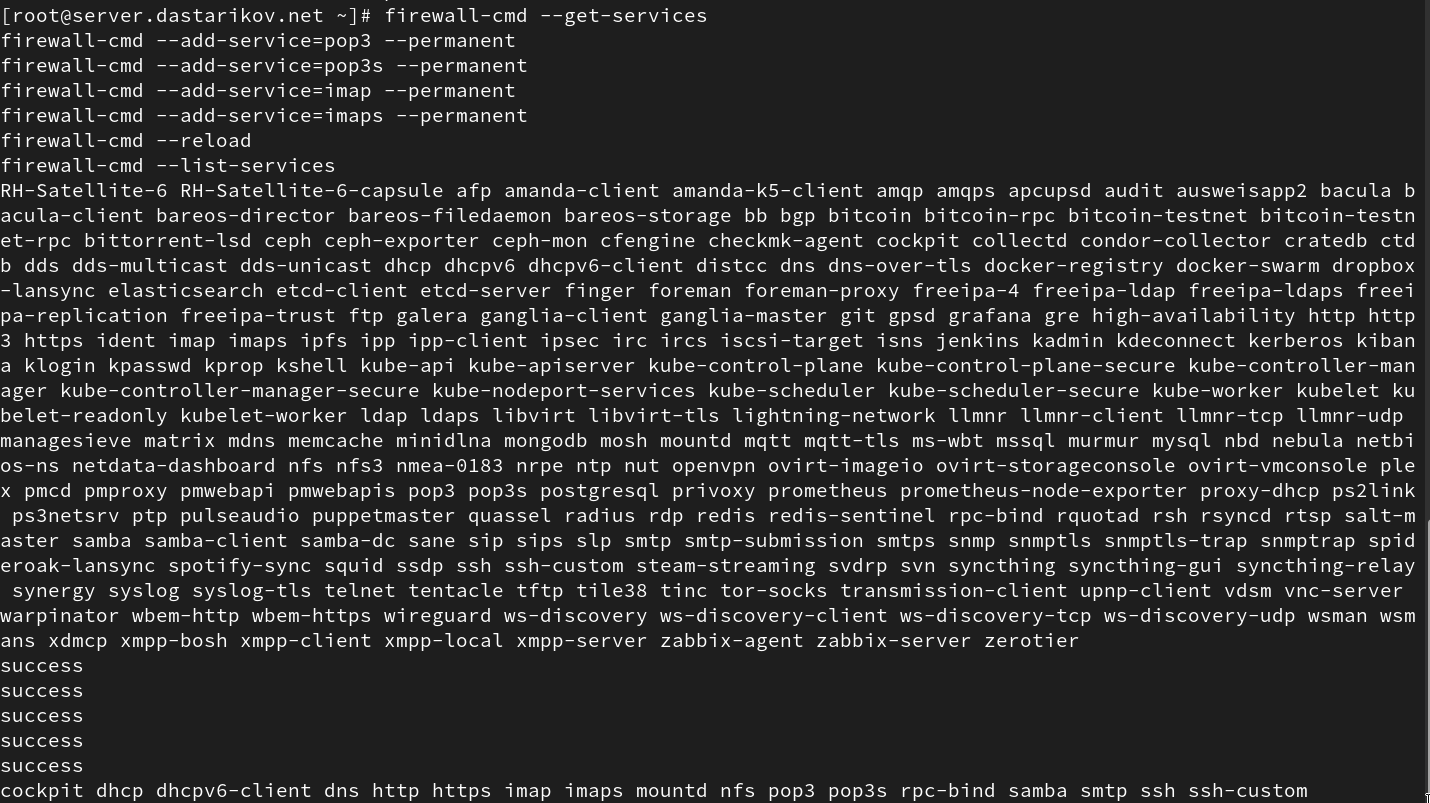
\includegraphics[width=\textwidth]{../images/image06.png}
    \captionof{figure}{Настройка межсетевого экрана для работы служб протоколов POP3 и IMAP.}
\end{frame}

\begin{frame}
\frametitle{Настройка Dovecot}
    \centering
    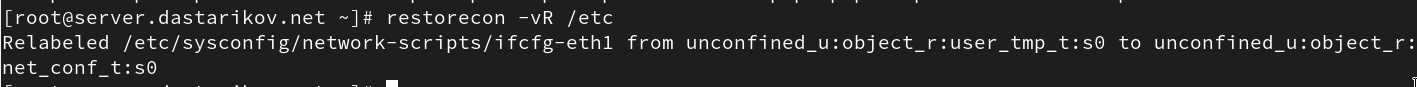
\includegraphics[width=\textwidth]{../images/image07.png}
    \captionof{figure}{Восстановление контекста безопасности в SELinux.}
\end{frame}

\begin{frame}
\frametitle{Настройка Dovecot}
    \centering
    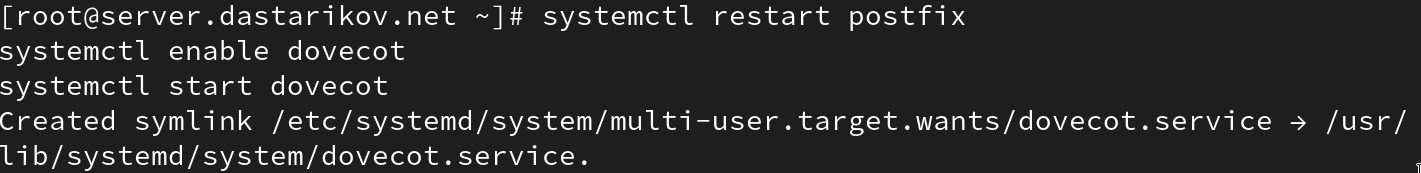
\includegraphics[width=\textwidth]{../images/image08.png}
    \captionof{figure}{Перезапуск Postfix и Dovecot.}
\end{frame}

\begin{frame}
\frametitle{Проверка работы Dovecot}
    \centering
    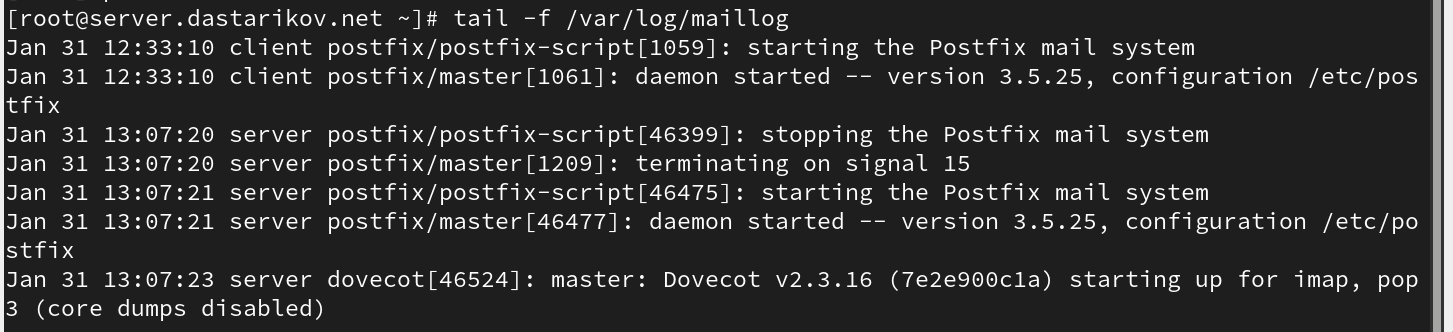
\includegraphics[width=\textwidth]{../images/image09.png}
    \captionof{figure}{Запуск мониторинга работы почтовой службы.}
\end{frame}

\begin{frame}
\frametitle{Проверка работы Dovecot}
    \centering
    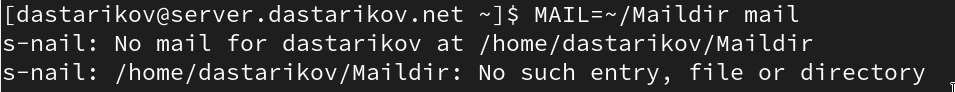
\includegraphics[width=\textwidth]{../images/image10.png}
    \captionof{figure}{Просмотр имеющейся почты на сервере.}
\end{frame}

\begin{frame}
\frametitle{Проверка работы Dovecot}
    \centering
    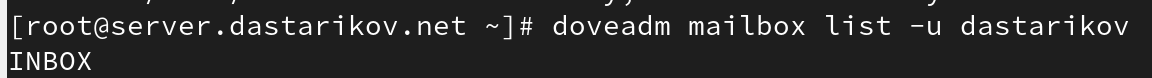
\includegraphics[width=\textwidth]{../images/image11.png}
    \captionof{figure}{Просмотр почты пользователя \texttt{dastarikov}.}
\end{frame}

\begin{frame}[fragile]
\frametitle{Проверка работы Dovecot}
Установили на машине клиента почтовый клиент \texttt{Evolution}:
\begin{minted}{bash}
    dnf -y install evolution
\end{minted}
    \centering
    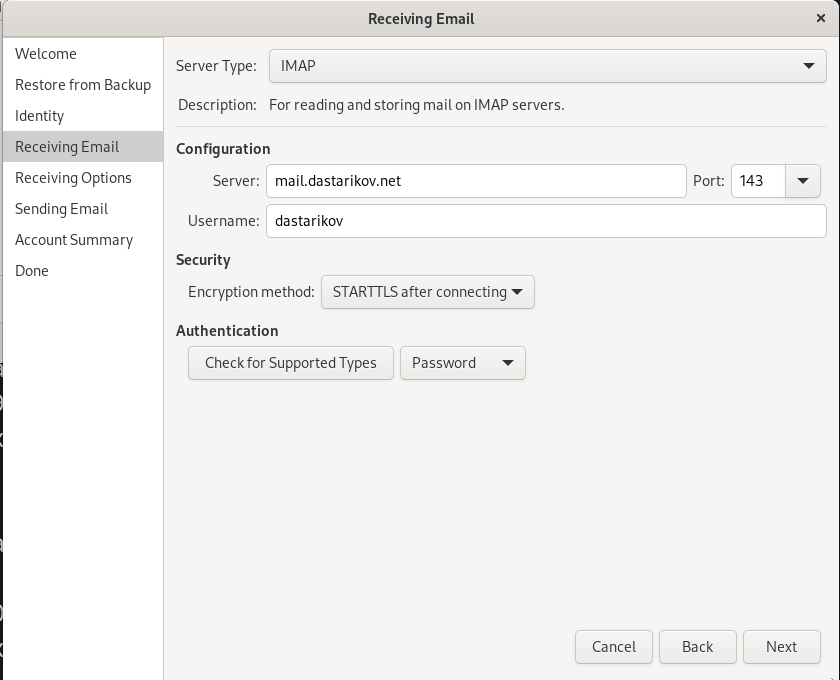
\includegraphics[width=0.8\textwidth]{../images/image12.png}
    \captionof{figure}{Настройка входящих сообщений.}
\end{frame}

\begin{frame}
\frametitle{Проверка работы Dovecot}
    \centering
    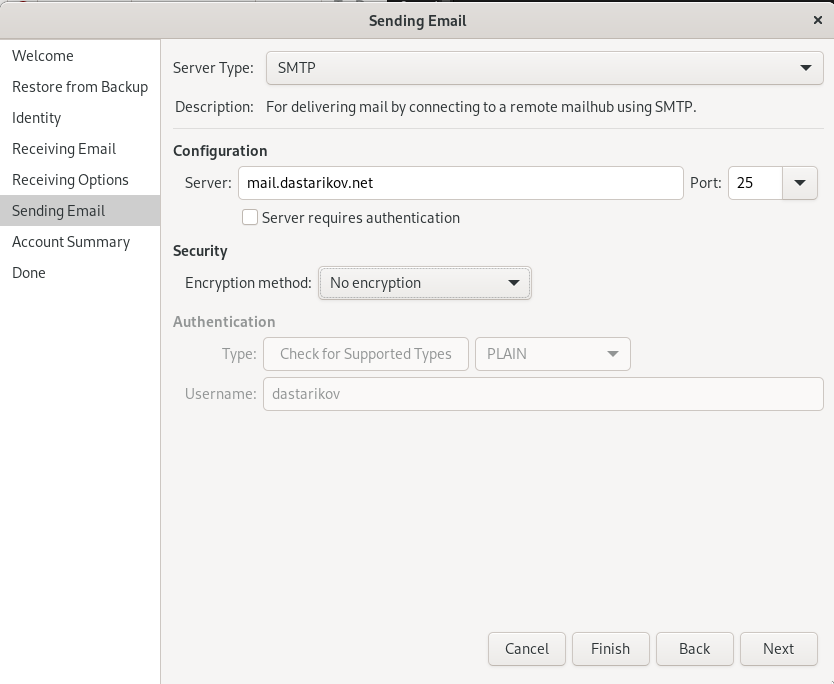
\includegraphics[width=0.8\textwidth]{../images/image13.png}
    \captionof{figure}{Настройка исходящих сообщений.}
\end{frame}

\begin{frame}
\frametitle{Проверка работы Dovecot}
    \centering
    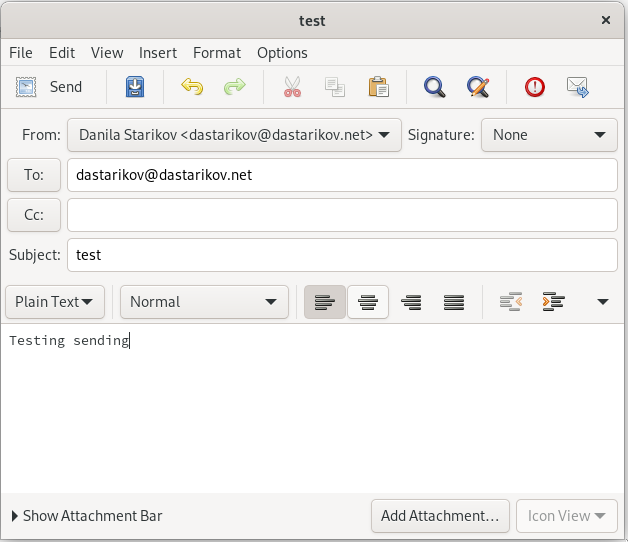
\includegraphics[width=0.8\textwidth]{../images/image14.png}
    \captionof{figure}{Окно отправки письма.}
\end{frame}

\begin{frame}
\frametitle{Проверка работы Dovecot}
    \centering
    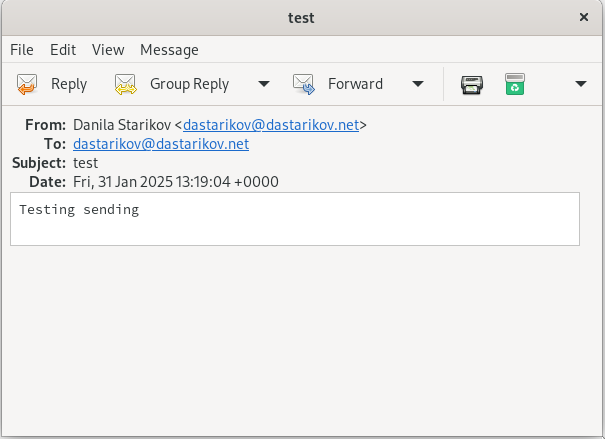
\includegraphics[width=\textwidth]{../images/image15.png}
    \captionof{figure}{Окна просмотра полученного письма.}
\end{frame}

\begin{frame}
\frametitle{Проверка работы Dovecot}
    \centering
    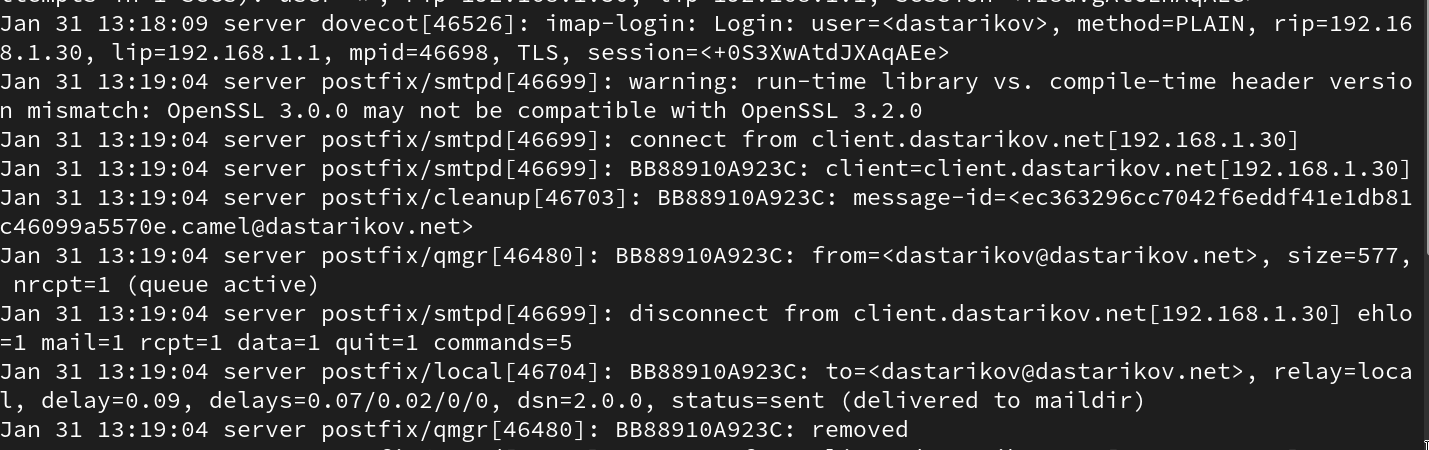
\includegraphics[width=\textwidth]{../images/image16.png}
    \captionof{figure}{Просмотр логов почтовой службы при отправке писем с клиента.}
\end{frame}

\begin{frame}
\frametitle{Проверка работы Dovecot}
    \centering
    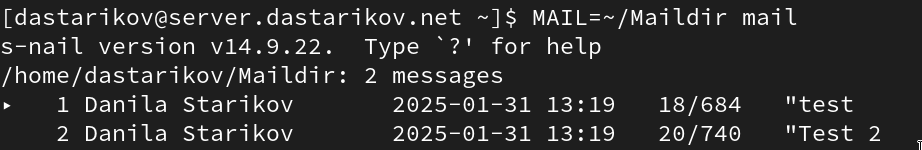
\includegraphics[width=\textwidth]{../images/image17.png}
    \captionof{figure}{Просмотр полученных писем через утилиту \texttt{mail}.}
\end{frame}

\begin{frame}
\frametitle{Проверка работы Dovecot}
    \centering
    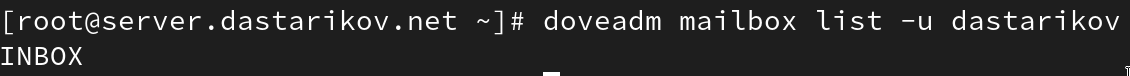
\includegraphics[width=\textwidth]{../images/image18.png}
    \captionof{figure}{Просмотр полученных писем через утилиту \texttt{doveadm}.}
\end{frame}

\begin{frame}
\frametitle{Проверка работы Dovecot}
    \centering
    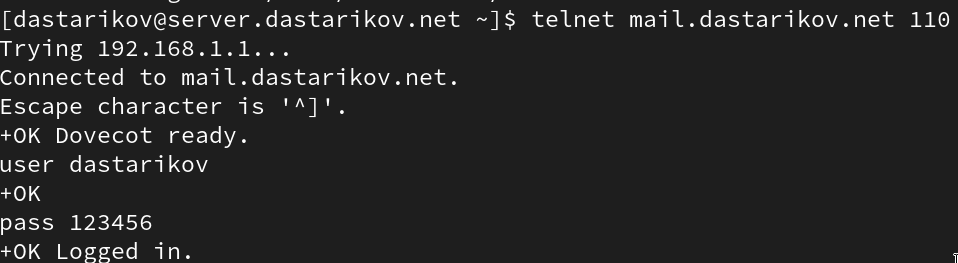
\includegraphics[width=\textwidth]{../images/image19.png}
    \captionof{figure}{Подключение к почтовому серверу через протокол Telnet.}
\end{frame}

\begin{frame}
\frametitle{Проверка работы Dovecot}
    \centering
    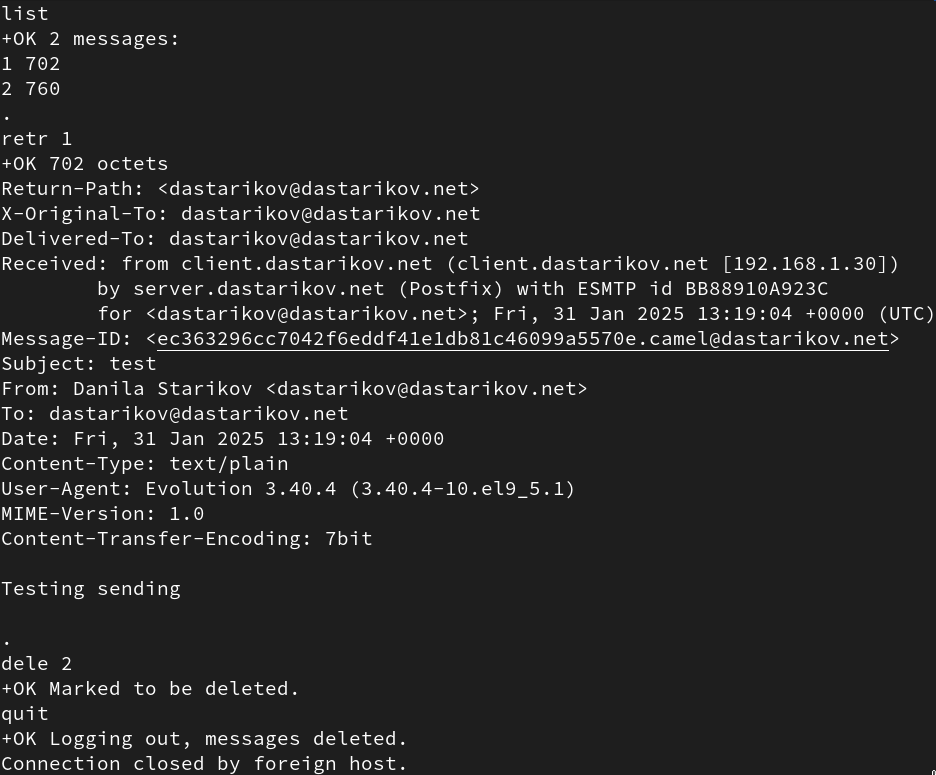
\includegraphics[width=0.8\textwidth]{../images/image20.png}
    \captionof{figure}{Работа с почтовым сервером через telnet.}
\end{frame}

\begin{frame}[fragile,containsverbatim]
\frametitle{Внесение изменений в настройки внутреннего окружения виртуальной машины}
\begin{minted}[breaklines,fontsize=\small]{bash}
  cd /vagrant/provision/server
  mkdir -p /vagrant/provision/server/mail/etc/dovecot/conf.d
  cp -R /etc/dovecot/dovecot.conf /vagrant/provision/server/mail/etc/dovecot/
  cp -R /etc/dovecot/conf.d/10-auth.conf /vagrant/provision/server/mail/etc/dovecot/conf.d/
  cp -R /etc/dovecot/conf.d/auth-system.conf.ext /vagrant/provision/server/mail/etc/dovecot/conf.d/
  cp -R /etc/dovecot/conf.d/10-mail.conf /vagrant/provision/server/mail/etc/dovecot/conf.d/
\end{minted}
\end{frame}

\begin{frame}[fragile,containsverbatim]
\frametitle{Внесение изменений в настройки внутреннего окружения виртуальной машины}
\begin{minted}[breaklines,fontsize=\small]{bash}
  dnf -y install dovecot
  dnf -y install telnet
  firewall-cmd --add-service pop3 --permanent
  firewall-cmd --add-service pop3s --permanent
  firewall-cmd --add-service imap --permanent
  firewall-cmd --add-service imaps --permanent
  firewall-cmd --add-service smtp-submission --permanent
  echo "Configure postfix for dovecot"
  postconf -e 'home_mailbox = Maildir/'
  echo "Configure postfix for auth"
  postconf -e 'smtpd_sasl_type = dovecot'
  postconf -e 'smtpd_sasl_path = private/auth'
  postconf -e 'smtpd_recipient_restrictions = reject_unknown_recipient_domain, permit_mynetworks, reject_non_fqdn_recipient, reject_unauth_destination, reject_unverified_recipient, permit'
  postconf -e 'mynetworks = 127.0.0.0/8'
\end{minted}
\end{frame}

\begin{frame}[fragile,containsverbatim]
\frametitle{Внесение изменений в настройки внутреннего окружения виртуальной машины}
\begin{minted}[breaklines,fontsize=\small]{bash}
  echo "Configure postfix for SMTP over TLS"
  cp /etc/pki/dovecot/certs/dovecot.pem /etc/pki/tls/certs
  cp /etc/pki/dovecot/private/dovecot.pem /etc/pki/tls/private
  postconf -e 'smtpd_tls_cert_file=/etc/pki/tls/certs/dovecot.pem'
  postconf -e 'smtpd_tls_key_file=/etc/pki/tls/private/dovecot.pem'
  postconf -e 'smtpd_tls_session_cache_database = btree:/var/lib/postfix/smtpd_scache'
  postconf -e 'smtpd_tls_security_level = may'
  postconf -e 'smtp_tls_security_level = may'
  postfix set-permissions
\end{minted}
\end{frame}

\begin{frame}
\frametitle{Выводы}
\begin{itemize}
    \item В результате выполнения лабораторной работы приобрели практические навыки по установке и простейшему конфигурированию POP3/IMAP-сервера.
\end{itemize}
\end{frame}
\end{document}
